\pdfminorversion=4

\documentclass{beamer}
\usepackage[utf8]{inputenc}
\usepackage[spanish]{babel}
%\usepackage[english]{babel}
\usepackage{graphicx}  % Graphics

\usepackage{beamerthemeULoyola}
\usepackage{graphicx}
\usepackage{booktabs}
\usepackage{blindtext}

%% PRESENTATION CONFIGURATION PARAMETERS %%%%%%%%%%%%%%%%%%%%%%%%%%%%%%%%%%%%%%%
\titlebackgroundfile{images/plantilla_portada}
\framebackgroundfile{images/plantilla_slide}
\definecolor{azulloyola}{HTML}{023E83}
\definecolor{azulloyolaclaro}{HTML}{9497B9}
\definecolor{gris}{HTML}{4C4C4C}
\definecolor{grisclaro}{HTML}{EBEBEB}
\definecolor{examplefrente}{HTML}{218E58}
\definecolor{examplefondo}{HTML}{C2D8CD}
\definecolor{alertfrente}{HTML}{FF0000}
\definecolor{alertfondo}{HTML}{E7BDBD}


\usefonttheme{structurebold}
\setbeamercolor{author in head/foot}{fg=white}
\setbeamercolor{title in head/foot}{fg=white}
\setbeamercolor{section in head/foot}{fg=azulloyola}
\setbeamercolor{normal text}{fg=gris}
\setbeamercolor{frametitle}{fg=azulloyola}
% \setbeamerfont{block title}{size={}}
\setbeamerfont{author}{size=\footnotesize}
\setbeamerfont{date}{size=\footnotesize}
\setbeamertemplate{itemize item}[circle]
\setbeamertemplate{itemize subitem}[triangle]
\setbeamertemplate{itemize subsubitem}[square]
\setbeamertemplate{itemize subsubsubitem}[ball]
\setbeamercolor{itemize item}{fg=azulloyola}
\setbeamercolor{itemize subitem}{fg=azulloyola}
\setbeamercolor{itemize subsubitem}{fg=azulloyola}
\setbeamercolor{itemize subsubsubitem}{fg=azulloyola}
\setbeamercolor{enumerate item}{fg=azulloyola}
\setbeamercolor{enumerate subitem}{fg=azulloyola}
\setbeamercolor{enumerate subsubitem}{fg=azulloyola}
\setbeamercolor{enumerate subsubsubitem}{fg=azulloyola}
% \setbeamercolor{alerted text}{fg=azulloyola}
% \setbeamerfont{alerted text}{series=\bfseries}

\setbeamertemplate{blocks}[shadow=true]
\setbeamercolor*{block title}{bg=azulloyolaclaro,fg=white}
\setbeamercolor*{block body}{bg=grisclaro,fg=gris}

\setbeamercolor*{block title example}{bg=examplefrente,fg=white}
\setbeamercolor*{block body example}{bg=examplefondo,fg=gris}

\setbeamercolor*{block title alerted}{bg=alertfrente,fg=white}
\setbeamercolor*{block body alerted}{bg=alertfondo,fg=gris}

\usecolortheme[named=azulloyola]{structure}


% This command makes that acrobat reader doesn't changes the colors of the slide
% when there are figures with transparencies.
\pdfpageattr {/Group << /S /Transparency /I true /CS /DeviceRGB>>}
%%%%%%%%%%%%%%%%%%%%%%%%%%%%%%%%%%%%%%%%%%%%%%%%%%%%%%%%%%%%%%%%%%%%%%%%%%%%%%%%

%      + Short title.               + Title which appears in the cover.
%      v                            v
\title[Short title]{Diversidad explícita en modelos de Ensembles de Extreme Learning Machine}
%       + Short author names which appear in the slides.
%       v
\author[Author]
{   % Author names which appear in the cover page.
    Carlos Perales-Gonz\'alez\inst{1}
}
%          + Short affiliation which appears in the slides.
%          v
\institute[ULOYOLA]
{   % Affiliation information which appears in the cover page.
    \begin{tabular}{c}
    \inst{1}Universidad Loyola Andaluc\'ia
    \end{tabular}
}
%     + Short acronym of the conference or date of the presentation.
%     v
\date
{   % Conference name which appears in the cover page.
	\today
}

\begin{document}
% Creates the cover page.
\frame{\titlepage}

\begin{frame}{Esquema}
\tableofcontents
\end{frame}


% 45 minutos
\section{Introducción} % 10 minutos

\subsection{Aprendizaje automático (Machine Learning)}
% 1
\frame[allowframebreaks]{\frametitle{Inteligencia artificial. Machine Learning}
	
	\textbf{Ciencia de la Computación}: aquella que estudia el diseño y la construcción de máquinas (computadoras) que resuelven problemas, y cuáles de estos problemas son tratables \cite{mitchell2006discipline}. Dentro de esta Ciencia, un área que acoge cada vez más importante es: el Aprendizaje Automático (\textit{Machine Learning}). \\
	
	\textbf{Aprendizaje Automático (\textit{Machine Learning})}: area de conocimiento que utiliza las Matemáticas para elaborar modelos que estudian qué puede ser predicho a través de los datos, con una serie de hipótesis de modelado, y con qué confiabilidad \cite{mitchell2006discipline}.
	
	\begin{figure}[H]
		\centering
		\label{fig:nested}
		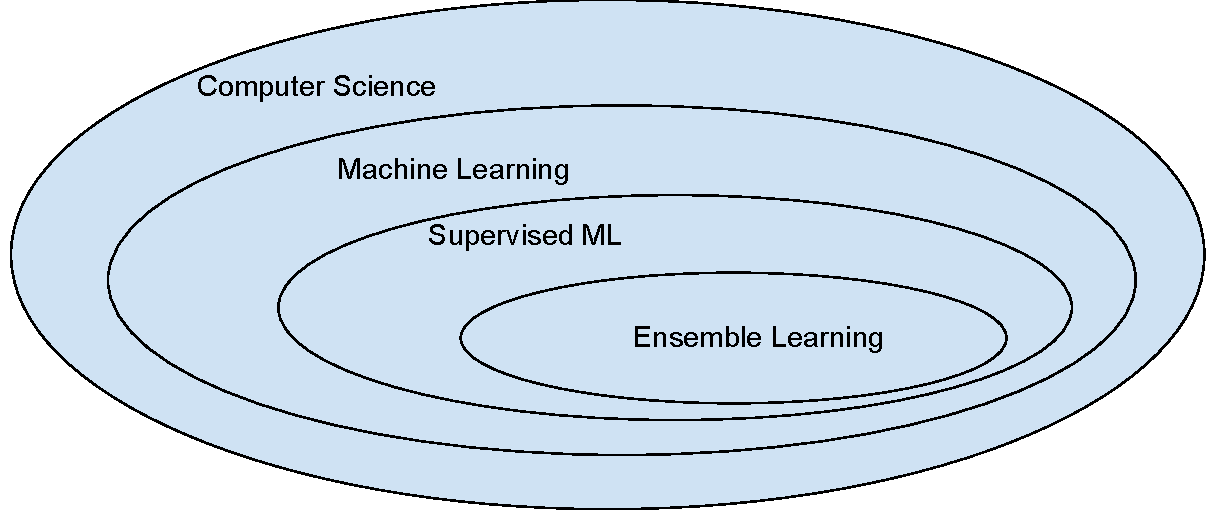
\includegraphics[scale=0.5]{images/nested.pdf}
%		\caption{Explicación del sesgo y la varianza como distancia al centro de una diana}
	\end{figure}

}

\subsection{Categorías del Aprendizaje Automático}

\frame{\frametitle{Machine Learning}

	\begin{itemize}
		\item Supervisado: se infiere una función que relacione variables de entrada (\textit{input variables}) y variables de salida (\textit{targets}), usando datos de situaciones previas donde estos datos pueden ser recogidos \cite{supervised_dict}.
		\begin{itemize}
			\item Regression: target numérico.
			\item Classificación: target categórico.
		\end{itemize}
		\item No supervisado: se infiere la estructura que tiene un conjunto de datos, en ausencia de un target o un feedback \cite{unsupervised_dict}. Los elementos son agrupados siguiendo relaciones entre las variables (\textit{Principal Component Analysis}, \textit{K-means}, $\ldots$).
		\item Por refuerzo:  busca aprender un patrón de comportamiento a través de problemas de toma de decisiones secuenciales con recompensas \cite{reinforcement_dict}.
	\end{itemize}
	
}

\frame[allowframebreaks]{
\frametitle{Supervised Machine Learning}

Conjunto de datos de entrenamiento $\mathcal{D} = \{  (\boldsymbol{x}_1, y_1), \ldots (\boldsymbol{x}_N, y_N) \} = \{ (\boldsymbol{x}_n, y_n) \}_{n=1}^N$. Buscamos un predictor $f : \mathcal{X} \rightarrow \mathcal{Y}$,


	\begin{figure}[H]
	\centering
	\label{fig:f}
	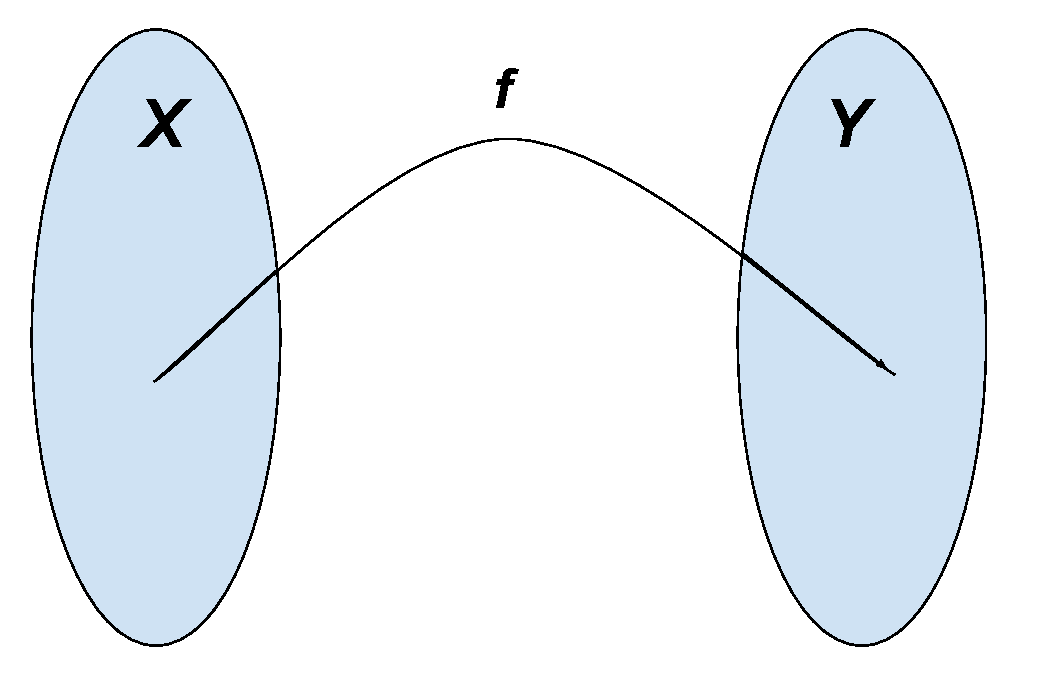
\includegraphics[scale=0.25]{images/f.pdf}
	%		\caption{Explicación del sesgo y la varianza como distancia al centro de una diana}
	\end{figure}

Hay muchos predictores posibles. Además, dependiendo del problema (regresión o clasificación), esa variable $y$ puede ser una variable numérica o categórica. Los problemas de clasificación se pueden convertir en multi-regresión a través del \textit{One-Hot-Encoding} \cite{one_hot_encoding}.


\begin{equation}
\label{eq:onehotencoding}
\boldsymbol{y}_{j, n} =
\begin{cases}
1 & \text{si } j \text{ es la clase a la que pertenece el patrón} n \\
0 & \text{en cualquier otro caso}
\end{cases}
\end{equation}

}
\frame{
En general, no podemos conocer exactamente la relación entre el dominio de las features, $\mathcal{X}$, y el dominio target, $\mathcal{Y}$. Sin embargo, podemos interpolar esos dominios a través de $n=1, \ldots, N$ patrones, con features $\boldsymbol{x}_n \in \mathcal{X}$, y target $\boldsymbol{y}_n \in \mathcal{Y}$.


\begin{equation}
\label{eq:f}
f (\boldsymbol{x}_n; \theta) \approx y_n, \: \forall n .
\end{equation}

Los predictores $f$ dependen de una serie de parámetros $\theta$. Para entrenar un predictor, optimizamos esos parámetros a través de la minimización del error cometido en predecir el set de entrenamiento $\mathcal{D}$.

\begin{equation}
\label{eq:omega_error}
\min_{\theta} \text{ Error} ( \left( f(\boldsymbol{x}_1; \theta ), y_1 \right), \ldots, \left( f(\boldsymbol{x}_N; \theta ), y_N \right) )
\end{equation}
}

\frame{
En problemas de regresión, clásicamente se utiliza el error cuadrático medio, o \textit{Mean Squared Error}, que es equivalente a calcular la norma $L2$ entre el target $y_n, \: n=1, \ldots, N$ y la predicción $f (\boldsymbol{x}_n), \:n=1, \ldots, N$.

\begin{equation}
\label{eq:mse}
\min_{\theta} \frac{1}{N} \sum_{n=1}^{N} { \left( f(\boldsymbol{x}_n; \theta ) - y_1 \right) }^2
\end{equation}


}

%\subsection{Dilema sesgo-varianza}
%
%\frame{\frametitle{Definición de sesgo y varianza}
%
%Explicación sesgo
%
%Explicación varianza
%
%}
%
%\frame{\frametitle{Sesgo, varianza y el MSE}
%	
%	Ecuación matemática con el MSE
%	
%}
%
%\frame{\frametitle{Ejemplo del sesgo y la varianza}
%	
%Ejemplo hecho con el Jupyter Notebook
%	
%}

\section{Ensemble Learning}

\frame[allowframebreaks]{\frametitle{Metodología ensemble}

\textit{Ensemble learning} es el proceso en el cual se entrenan diferentes predictores y se combinan sus salidas, tratando a esta arquitectura como un comité de decisores \cite{ensemble}.


\begin{figure}[H]
	\centering
	\label{fig:ensemble}
	\includegraphics[scale=0.3]{images/f_ensemble.pdf}
	%		\caption{Explicación del sesgo y la varianza como distancia al centro de una diana}
\end{figure}


Motivado por

\begin{itemize}
	\item \textbf{Problema de los datos} %: para entrenar los predictores, se utilizan distintas herramientas matemáticas orientadas a minimizar el error entre la predicción de los datos que tenemos para entrenar y la etiqueta que estos datos tienen. Se utilizan datos previamente recogidos para, en situaciones futuras, prever cuál será el comportamiento del sistema que estamos estudiando. Esta hipótesis (\textit{en el pasado ocurrió esto, luego en situaciones futuras ocurrirá lo mismo}) no está exenta de riesgo, y puede presentar algunos problemas:
	
	\begin{itemize}
		\item \textit{La muestra es pequeña o no concluyente} %: los datos, por lo general, no establecen una relación perfecta entre variables de entrada y de salida, puesto que a menudo se encuentran perturbado por un pequeño ruido, que a veces se puede modelar como un ruido $\epsilon$ proveniente de una distribución estadística \cite{noise}. Por esto mismo, incluso obtener subconjuntos de datos de todo el conjunto que se dispone para entrenamiento puede llevar a modelos distintos \cite{Bbeiman1996}. En esta línea, Laplace ya demostró en 1818 que la media aritmética de una muestra de datos provenientes de una distribución estadística no siempre representaba la media de la distribución original \cite{de1818theorie}.
		
		\item \textit{Las variables de entrada no son suficientes} %: otro problema asociado a los datos es que las variables de entrada no sean suficientes para explicar el modelo. Por ejemplo, en Meteorología ocurre el siguiente problema: si pudiésemos conocer el comportamiento de todas las partículas de aire del planeta y caracterizarlas, los modelos de predicción del tiempo atmosférico serían mucho más preciso. Sin embargo, no se dispone de esta información, pero sí de variables meteorológicas como la temperatura de una masa de aire, su velocidad y su presión atmosférica. Con estas variables, se crean modelos del tiempo atmosférico, pero son una simplificación de la realidad (todas las partículas influyen en el tiempo atmosférico, en mayor o menor medida) y este \textit{colapso de las variables} produce que los modelos no sean precisos.
	\end{itemize}
	
	\item \textbf{Problema de los modelos} %: además de los errores del modelo producidos a causa de los datos, los predictores presentan también sus propios problemas. No hay que olvidar que los predictores, como se explica en la Sección \ref{sec:supervised}, se obtienen a partir de una minimización de una expresión matemática del error, y como resultado el conjunto de parámetros $\Omega$ que caracteriza ese predictor $f ( \cdot, \Omega )$ \textit{se entrena} y se ajusta al comportamiento esperado según los datos. Esta hipótesis es bastante fuerte, y generalmente no se cumple totalmente:
	
	\begin{itemize}
		\item \textit{Los modelos no son suficientemente complejos} %: La hipótesis anteriormente mencionada (\textit{un predictor $f ( \cdot, \Omega )$ puede entrenarse de manera que, a partir de unas variables de entrada, se obtenga la variable de salida deseada}) se ve comprometida cuando el predictor carece de la representatividad que se le supone. En general, los problemas del mundo real son no-lineales: la variación de una variable de entrada no repercute exactamente en un múltiplo de esa variación para el valor de salida. Es más, en distintas regiones de la variable de entrada puede no verse afectada de misma manera la variable de salida. Por ejemplo, si se duplicar la superficie en metros cuadrados de una casa no tiene porqué duplicarse exactamente el precio de esta. Es más, el aumento del precio de $40$ a $80$ $m^2$ no tiene por qué ser el mismo que de $80$ a $160$ $m^2$. La respuesta entre las variables de entrada y de salida no tienen por qué ser proporcionales (ni inversamente proporcionales), y es por esto por lo que la mayoría de predictores son no-lineales (redes neuronales, kernel SVM, \ldots). Incluso presentando no-linealidad, puede que estos predictores no sean lo suficientemente complejos para capturar la no-linealidad de las relaciones entre las variables de entrada y de salida.
		
		\item \textit{El tiempo de aprendizaje crece \emph{ad eternum}} %: La complejidad de un predictor no está exenta de coste computacional. Al contrario, los modelos más complejos tienden a ser computacionalmente más costosos, y esto se suele traducir en un tiempo mayor de entrenamiento. Por esto, depende de cómo crezca el tiempo de computación, en los problemas de Aprendizaje Supervisado se pueden optar por modelos peor entrenados, si el error de minimización llega a una tolerancia dada. Además, con las técnicas de entrenamiento de conjunto, muchos predictores poco fiables, o predictores débiles (\textit{weak learners}) pueden ser acomplados como un comité de expertos, mejorando su predicción \cite{Freund1999}.
	\end{itemize}
\end{itemize}

Se construyen varios predictores, y se promueve la diversidad de distintas formas \cite{ye2012empirical}:

\begin{itemize}
	\item \textbf{Diversidad a través del kernel}: algunos predictores, como a regresión lineal o el SVM, no son netamente predictores no-lineales. Se pueden usar distintas funciones de mapeo no lineales \cite{theodoridis2009pattern}. % La no-linealidad se añade a trevés de una funciones de mapeo no lineales, que transforman el espacio original de las variables de entrada de los datos a un espacio transformado. Usando la herramienta matemática conocida como \textit{kernel trick}, las distancia entre los elementos del entrenamiento se ven modificadas explícitamente a través de una función kernel, de manera que implícitamente se añaden al modelo funciones de mapeo no lineales \cite{theodoridis2009pattern}. Como las funciones kernel y la forma de incluirlas en los modelos no son únicas, diferentes predictores se pueden generar variando estas funciones kernel.
	
	\item \textbf{Diversidad a través de los datos}: distintos subconjuntos de un conjunto de datos no tienen por qué llevar el mismo predictor. De esta categoría del entrenamiento de conjunto surge las familias más importantes de meta-algoritmos, Bagging \cite{Bbeiman1996} and Boosting \cite{Freund1999}. % es el ejemplo más conocido de la metodología Boosting, que resulta en seleccionar los subconjuntos de datos de entrenamiento basados en el rendimiento de los predictores. De un predictor al siguiente, los patrones en los datos que no son clasificados correctamente adquieren más importancia, de manera que el siguiente predictor que se añada al comité tiende a eliminar esta predicciones erróneas \cite{Hastie2009}. Por otro lado está la metodología Bagging, que es la contracción de \textit{bootstrap aggregating}  \cite{Bbeiman1996}. Esta metodología genera distintos predictores a través de la selección de subconjuntos del entrenamiento. Estos subconjuntos se tratan como conjuntos de datos independientes, usados para entrenar distintos predictores \cite{Zhao2012}.
	
	\item \textbf{Diversidad a través de parámetros}: esta categoría incluye métodos de generación de predictores en los cuales se utilizan parámetros durante el periodo de entrenamiento. Por ejemplo, El Aprendizaje de Correlación Negativa (\textit{Negative Correlation Learning}) \cite{liu1999ensemble}. % Como se comentó al final de la Sección \ref{sec:supervised}, existen parámetros que no son optimizados directamente en el entrenamiento: el número de neuronas y de capas en las redes neuronales, el número de hojas y la profundidad de los árboles de decisión, el parámetro de margen en los SVMs, \ldots  La modificación de estos parámetros puede llevar a predictores diversos entre sí. Además, algunas metodologías como el Aprendizaje de Correlación Negativa (\textit{Negative Correlation Learning}) incluyen parámetros extra en los procesos de entrenamiento para poder generar predictores diversos de manera controlada \cite{Liu1999}.
\end{itemize}



}

%\frame{\frametitle{Metodología boosting}
%
%Ejemplo de la carrera de caballos (artículo original del Adaboost).
%
%}
%
%\frame{\frametitle{Metodología bagging}
%	
%Buscar ejemplo
%	
%}


\frame{\frametitle{Ventajas-desventajas del data sampling}

La principal hipótesis de éstos métodos es que distintos subsets de datos generan predictores diversos entre sí \cite{Ko2008}. \\


\textbf{Ventaja:}	
Es fácil de adaptar a cualquier algoritmo. No modifica \textit{la caja negra}, es externo. \\


\textbf{Desventaja:}
Depende en la heterogeneidad de los datos. Hay que tener muchos datos y que cada subset del conjunto de entrenamiento sea diverso entre sí. \\
	
}


\section{Extreme Learning Machine}  % 5 minutos

\frame[allowframebreaks]{\frametitle{Extreme Learning Machine}

El predictor es de la siguiente forma:
	
	\begin{equation}
		\label{eq:elm}
		f(\boldsymbol{x}) = h(\boldsymbol{x})' \boldsymbol{\beta}
	\end{equation}
	
Donde:
	
\begin{itemize}
	\item $\boldsymbol{x} \in \mathbb{R}^K$.
	\item $y \in R$.
	\item $h: \mathbb{R}^K \rightarrow \mathbb{R}^D$.
	\item $\boldsymbol{\beta} \in \mathbb{R}^{D \times 1}$.
\end{itemize}

	
	\begin{figure}[H]
		\centering
		\label{fig:elm}
		\includegraphics[scale=0.5]{images/ELM.pdf}
		%		\caption{Explicación del sesgo y la varianza como distancia al centro de una diana}
	\end{figure}

Y el problema de minimización asociado es


\begin{equation}
	\min_{\boldsymbol{\beta}} {\lVert \boldsymbol{H} \boldsymbol{\beta} - \boldsymbol{Y} \rVert}_2^2 + C {\lVert \boldsymbol{\beta} \rVert}_2^2.
\end{equation}

Donde:

\begin{itemize}
	\item ${\lVert \cdot \rVert}_2$ es la norma $L2$.
	\item $\boldsymbol{H} = \left(\boldsymbol{h}' \left(\boldsymbol{x}_{1}\right), \ldots, \boldsymbol{h}' \left(\boldsymbol{x}_{N}\right)\right)'$.
	\item $Y = (y_1, \ldots, y_N)'$. 
\end{itemize}

Y la solución es:

\begin{equation}
\label{eq:solucion_elm}
\boldsymbol{\beta} = \left( \boldsymbol{H}' \boldsymbol{H} + C \boldsymbol{I} \right)^{-1} \boldsymbol{H}' \boldsymbol{Y}
\end{equation}
}


\section{Promoción de la diversidad explícita en ELM}  % 20 minutos
\subsection{RE-ELM}

\frame[allowframebreaks]{\frametitle{RE-ELM}
}

\subsection{NC-ELM}

\frame[allowframebreaks]{\frametitle{RE-ELM}
}

\subsection{GNC-ELM}

\frame[allowframebreaks]{\frametitle{RE-ELM}
}

\section{Conclusiones} % 5 minutos

\frame[allowframebreaks]{

\begin{enumerate}
	\item \textit{REELM} \cite{reelm}.El primer elemento del conjunto es el ELM tradicional sin diversidad incluida. El segundo predictor se añade con la diversidad con respecto al primer elemento. El tercer predictor, tiene añadidas la diversidad con respecto al primero y al segundo elemento del conjunto, y así sucesivamente. Por este motivo, decimos que en el conjunto existe una jerarquía. %, pues el primer predictor es el ELM y los demás se añaden como perturbaciónes al sistema. De hecho, el peso que tienen en la combinación lineal final (Ecuación \eqref{eq:alpha_s}) es cada vez menor.
	
	\item \textit{NCELM} \cite{ncelm}. Para la segunda propuesta, la diversidad no se aplica progresivamente a los predictores del conjunto, sino que todos tienen el mismo término de la diversidad.% Primero, los distintos predictores se generan modificando los pesos de la capa de entrada, resultando en distintos funciones de mapeo no lineales para los datos. Como se ha comentado en la Sección \ref{sec:diversity}, esto genera diversidad implícita, pero no se controla la diversidad en las predicciones. Por eso, posteriormente la diversidad se incluye en el problema de minimización de todos los predictores. Este término es el cuadrado del producto escalar de su predicción sobre el conjunto de datos y la predicción del conjunto de predictores. 
	
	El término de la diversidad es el mismo para todos los predictores y estos están igualmente pesados en la combinación final del conjunto. Establecer primero una diversidad implícita para luego explícitamente promoverla permite eliminar la jerarquía de la propuesta \textit{RE-ELM}.
	
	\item \textit{GNCELM} \cite{gncelm}. Aunque la propuesta anterior elimina la jerarquía, necesita primero generar los predictores y luego actualizarlos iterativamente. El conjunto de predictores no se obtienen en $S$ entrenamientos, siendo $S$ el número de predictores, sino $S$ por $iter$, siendo $iter$ las iteraciones que se realizaban en el conjunto. La propuesta \textit{GNCELM} considera el conjunto como un único predictor con muchas pequeñas partes que componen la solución final. La reducción del error se hace no teniendo en cuenta las predicciones individuales, sino el conjunto de predictores. De esta manera, existe un único entrenamiento global, del cual obtenemos los coeficientes de los pesos para todos los \textit{ELM} que forman el conjunto.
\end{enumerate}

Las propuestas metodológicas de esta tesis apunta a mantener las mejoras de cada una de las propuestas anteriores, al mismo tiempo que intenta reducir sus ventajas. El último artículo de la tesis \cite{gncelm} además explica matemáticamente la importancia de minimizar el el error del conjunto y no de los predictores. Por ello, la exposición matemática que se realiza abre la puerta a exportar esta propuesta metodológica a otros modelos distintos de \textit{Extreme Learning Machine}.

}


% END
\section*{END}
\frame{
	\frametitle{END}
\begin{center}
	\huge GRACIAS
\end{center}
}

% BIBLIOGRAPHY
\section*{Bibliography}
\begin{frame}[allowframebreaks]
	\frametitle{References}
    \bibliographystyle{ieeetr}
	\bibliography{references.bib}
\end{frame}


\end{document}
